\subsection{Setup 2 - Fuzzy C-Means: Resultados nos Datasets Adult e Dry Bean}

Neste setup, avaliamos o desempenho do Fuzzy C-Means supervisionado nos conjuntos Adult (balanceado) e Dry Bean (balanceado), ambos após pré-processamento e balanceamento por oversampling. O pipeline seguiu as etapas de normalização, divisão estratificada, definição do número de clusters, treinamento, repetição dos experimentos (30 execuções) e análise quantitativa.

\subsubsection{Adult (Balanceado)}

O Fuzzy C-Means foi executado com $n_{clusters}=8$. Os resultados médios das 30 repetições estão na Tabela~\ref{tab:cmeans_adult_metrics}.

% Tabela Adult apenas acurácia e desvio padrão
\begin{table}[H]
\centering
\caption{Resultados quantitativos do Fuzzy C-Means no dataset Adult (balanceado, $n_{clusters}=8$)}
\label{tab:cmeans_adult_metrics}
\begin{tabular}{lcc}
\toprule
Métrica & Média & Desvio Padrão \\
\midrule
Acurácia & 0.7259 & 0.0034 \\
\bottomrule
\end{tabular}
\end{table}

As principais visualizações estão apresentadas a seguir:
\begin{figure}[ht]
    \centering
    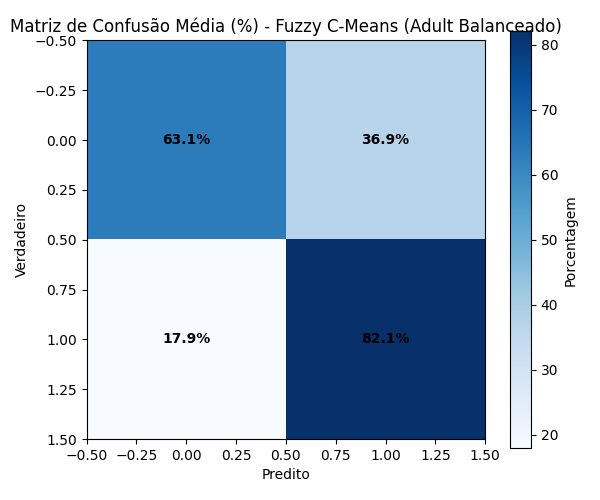
\includegraphics[width=0.7\linewidth]{../src/img/cmeans_adult_balance_confusion_matrix_media_percent.png}
    \caption{Matriz de confusão (Fuzzy C-Means - Adult Balanceado)}
    \label{fig:cmeans_adult_balance_confusion_matrix}
\end{figure}
\begin{figure}[ht]
    \centering
    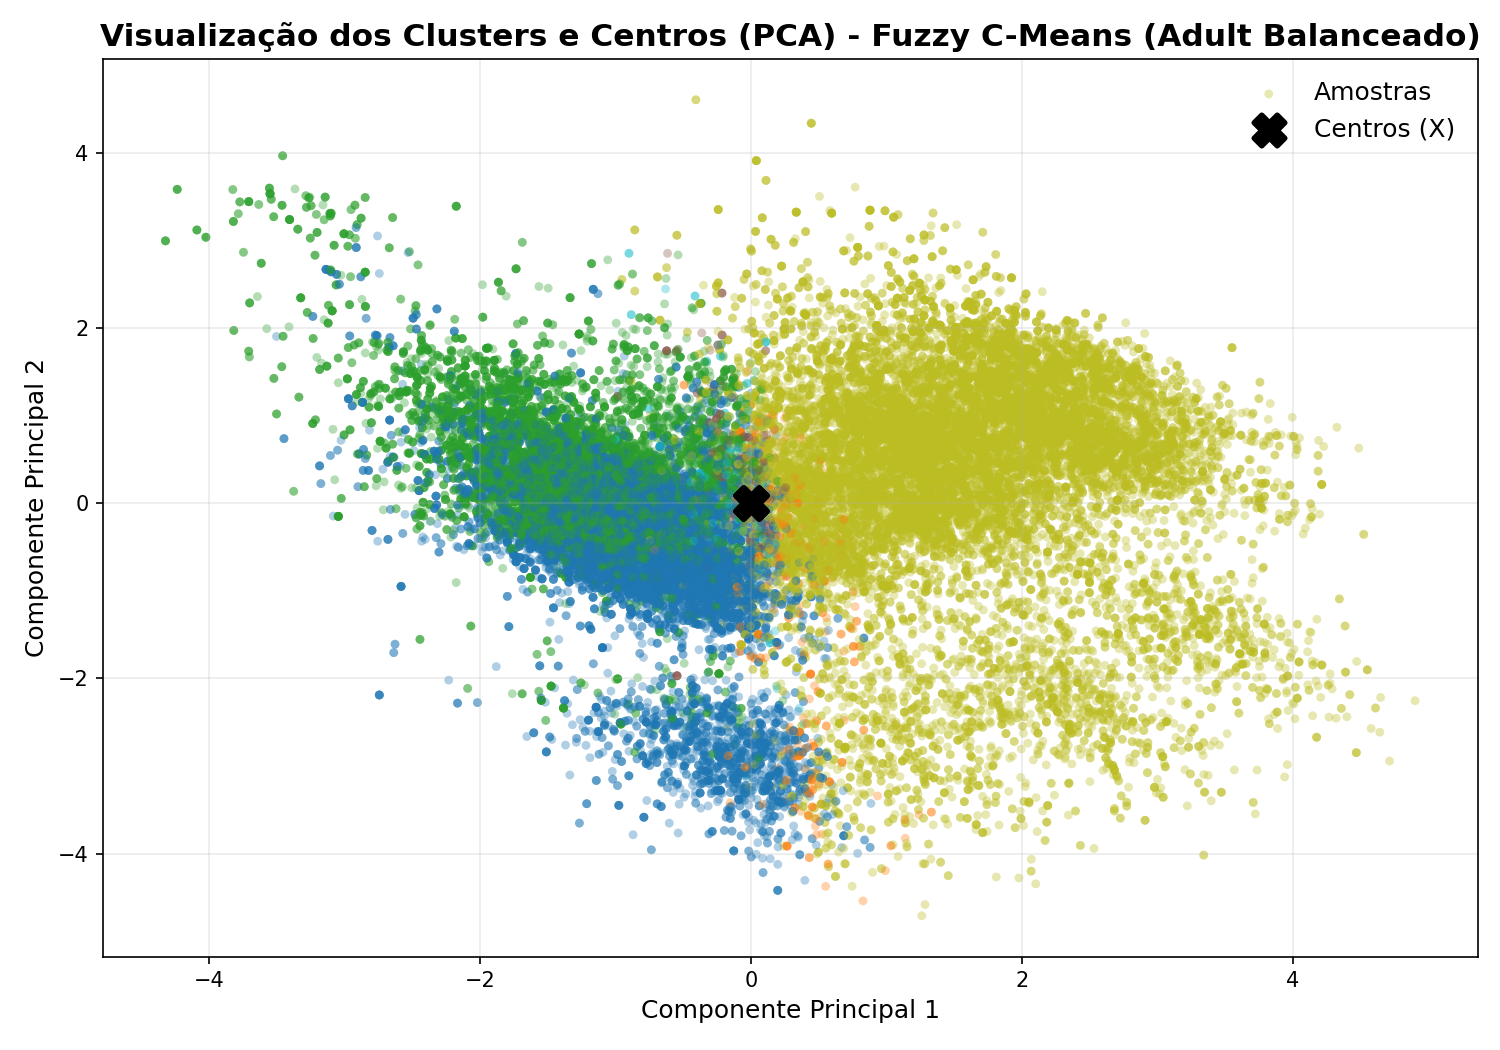
\includegraphics[width=0.7\linewidth]{../src/img/cmeans_adult_balance_clusters_pca.png}
    \caption{Visualização PCA dos clusters e centros (Fuzzy C-Means - Adult Balanceado)}
    \label{fig:cmeans_adult_balance_clusters_pca}
\end{figure}
\begin{figure}[ht]
    \centering
    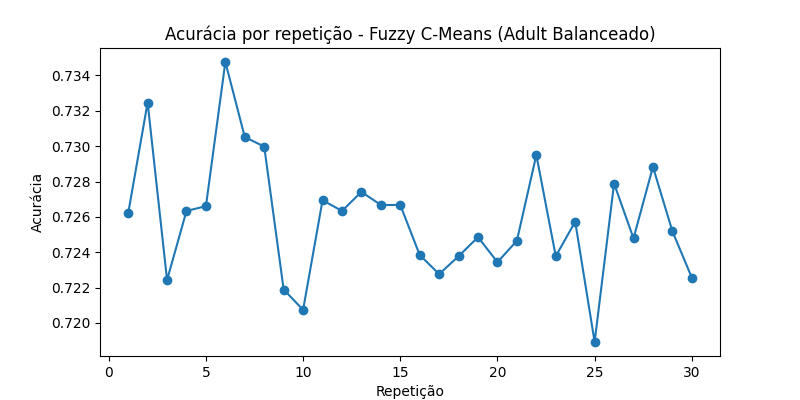
\includegraphics[width=0.7\linewidth]{../src/img/cmeans_adult_balance_accuracy_repetitions.png}
    \caption{Acurácia por repetição (Fuzzy C-Means - Adult Balanceado)}
\end{figure}
\begin{figure}[ht]
    \centering
    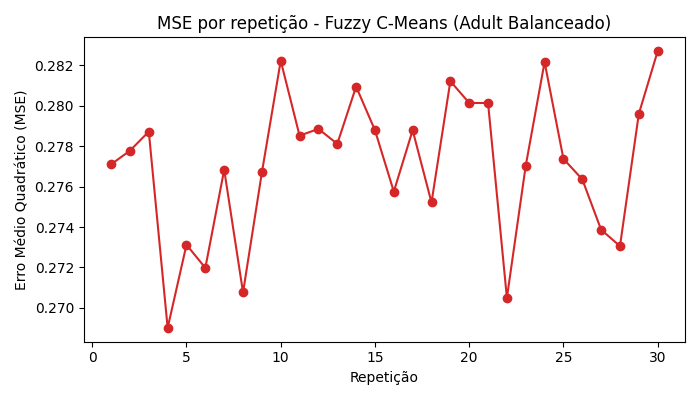
\includegraphics[width=0.7\linewidth]{../src/img/cmeans_adult_balance_mse_repetitions.png}
    \caption{MSE por repetição (Fuzzy C-Means - Adult Balanceado)}
\end{figure}

\subsubsection{Dry Bean (Balanceado)}

No dataset Dry Bean, o Fuzzy C-Means foi executado com $n_{clusters}=7$ e 30 repetições. Os resultados estão sumarizados na Tabela~\ref{tab:cmeans_drybean_metrics}.

% Tabela Dry Bean apenas acurácia e desvio padrão
\begin{table}[H]
\centering
\caption{Resultados quantitativos do Fuzzy C-Means no dataset Dry Bean (balanceado, $n_{clusters}=7$)}
\label{tab:cmeans_drybean_metrics}
\begin{tabular}{lcc}
\toprule
Métrica & Média & Desvio Padrão \\
\midrule
Acurácia & 0.8424 & 0.0205 \\
\bottomrule
\end{tabular}
\end{table}

As principais visualizações estão apresentadas a seguir:
\begin{figure}[ht]
    \centering
    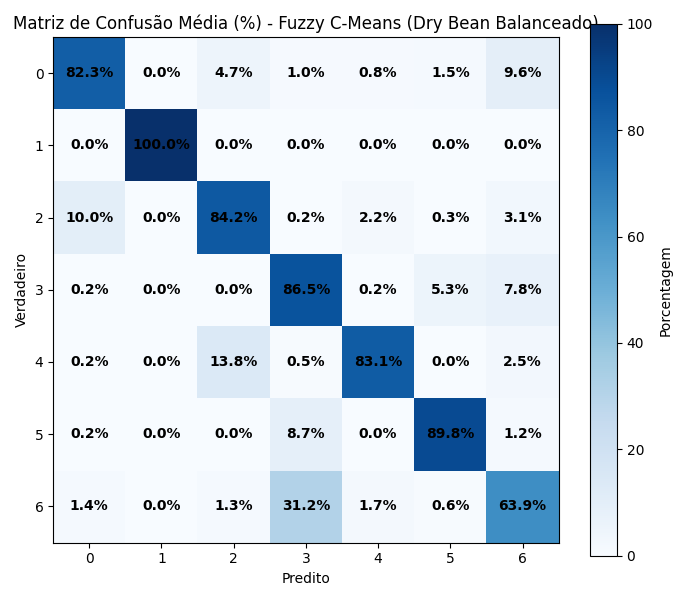
\includegraphics[width=0.7\linewidth]{../src/img/cmeans_drybean_balance_confusion_matrix_media_percent.png}
    \caption{Matriz de confusão (Fuzzy C-Means - Dry Bean Balanceado)}
    \label{fig:cmeans_drybean_balance_confusion_matrix}
\end{figure}
\begin{figure}[ht]
    \centering
    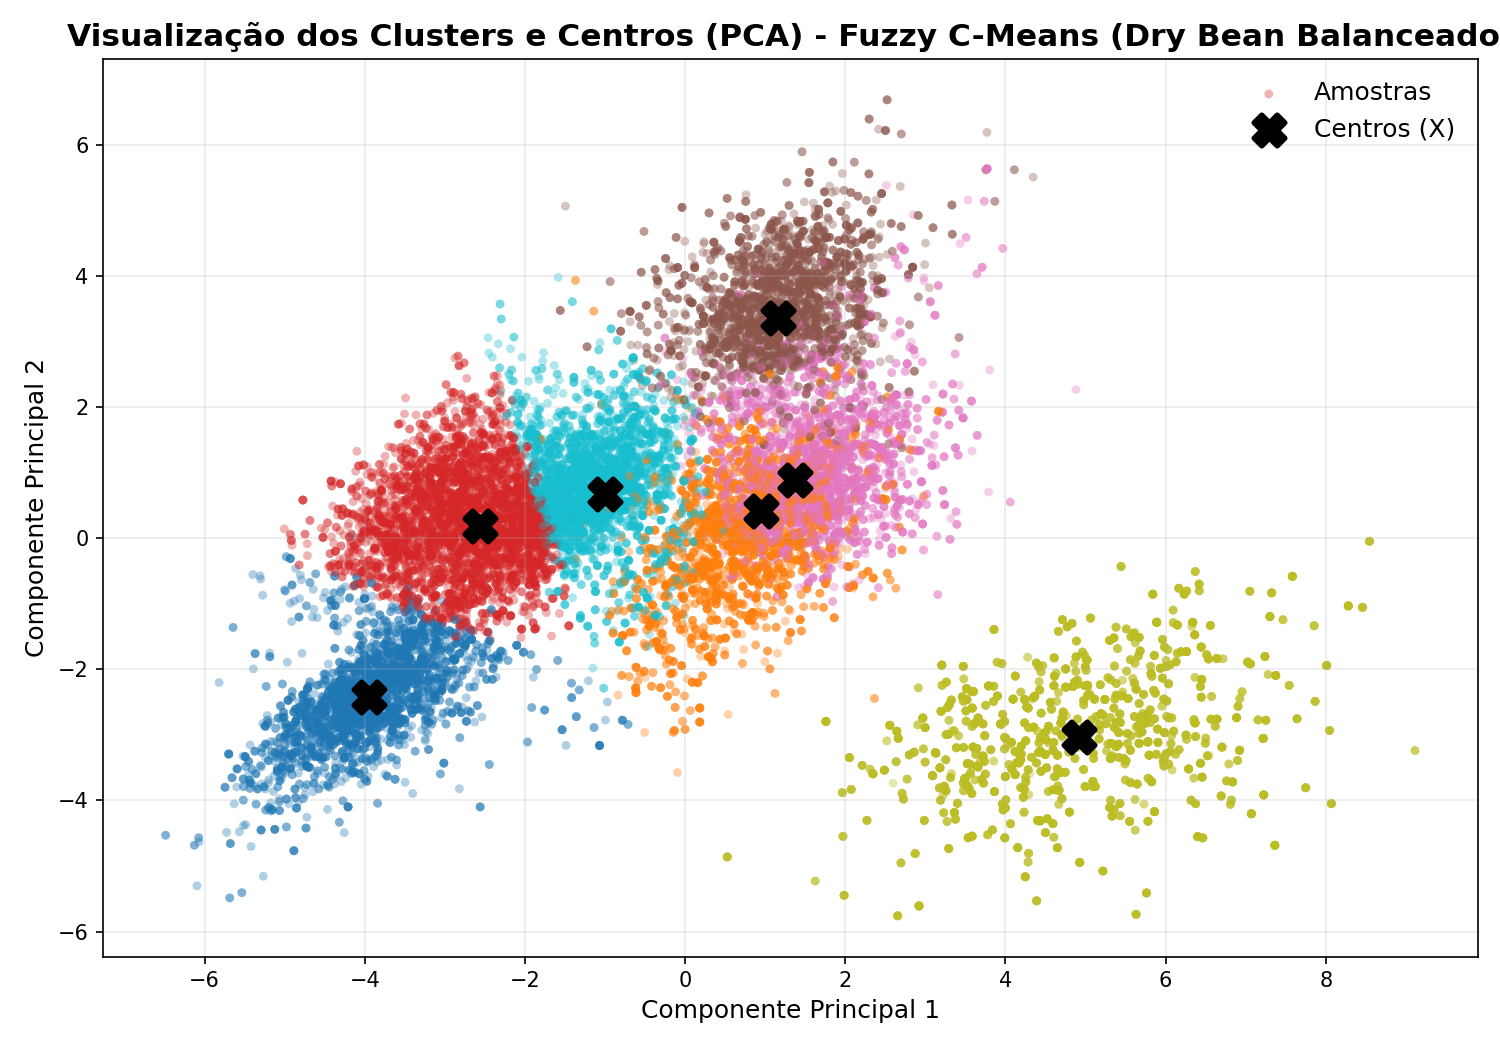
\includegraphics[width=0.7\linewidth]{../src/img/cmeans_drybean_balance_clusters_pca.png}
    \caption{Visualização PCA dos clusters e centros (Fuzzy C-Means - Dry Bean Balanceado)}
    \label{fig:cmeans_drybean_balance_clusters_pca}
\end{figure}
\begin{figure}[ht]
    \centering
    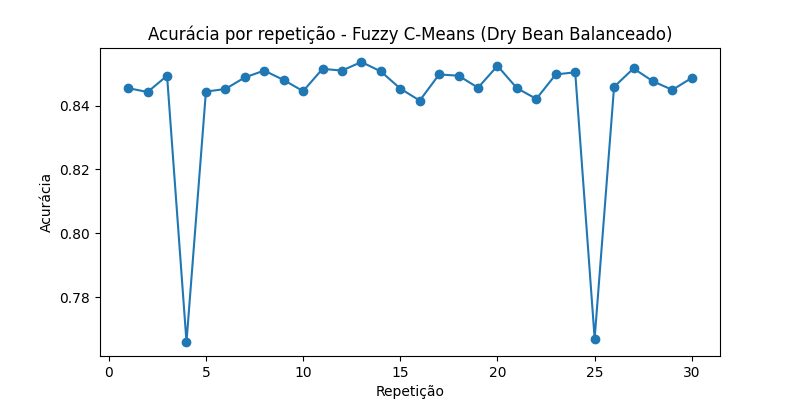
\includegraphics[width=0.7\linewidth]{../src/img/cmeans_drybean_balance_accuracy_repetitions.png}
    \caption{Acurácia por repetição (Fuzzy C-Means - Dry Bean Balanceado)}
\end{figure}
\begin{figure}[ht]
    \centering
    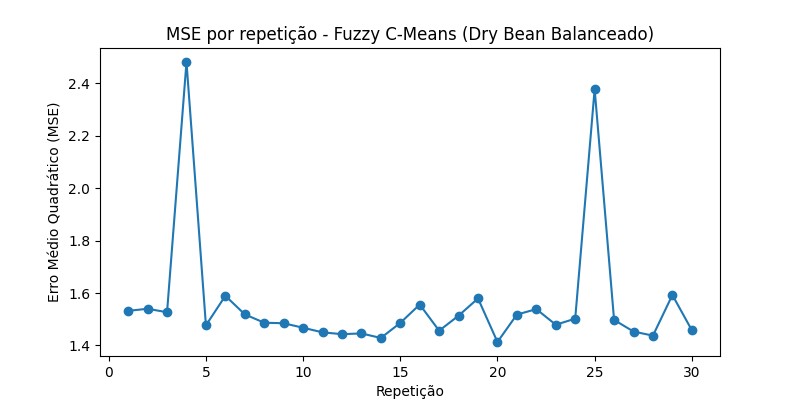
\includegraphics[width=0.7\linewidth]{../src/img/cmeans_drybean_balance_mse_repetitions.png}
    \caption{MSE por repetição (Fuzzy C-Means - Dry Bean Balanceado)}
\end{figure}
